\chapter{\label{chap:grundlagen}Grundlagen}
Dieses Kapitel befasst sich mit sowohl den mathematischen als auch den technischen Grundlagen der zu behandelnden Thematik, welche für das weitere Verständnis der Arbeit beitragen.
% -------------------------------------------------
% TECHNISCHE GRUNDLAGEN
% -------------------------------------------------
\section{\label{sec:technGrundlagen}Technische Grundlagen}
Im Zuge dieser Arbeit wird eine Smartphone Anwendung erstellt, deren Grundlage für die Implementierung die Software-Plattform Android und der im \gls{Smartphone} integrierte \gls{GPS}-Sensor ist. Die eigene Position und Geschwindigkeit wird mittels \gls{GPS} ermittelt, um in Verbindung mit der festen Position der nächsten \gls{LSA} die optimale Geschwindigkeit für das Erreichen der "'Grünen Welle"' zu errechnen. Im folgenden Abschnitt werden Funktionsweise und Besonderheiten der verwendeten Technologien beschrieben. 
% ANDROID
\subsection{Android}
Android ist ein von Google entwickeltes Linux-basiertes Betriebssystem für Mobilgeräte. 
Android-Anwendungen werden mit der Programmiersprache Java und der Auszeichnungssprache \gls{XML} entwickelt. Mit dem Android \gls{SDK}\footnote{ Das Android \gls{SDK} steht unter \url{https://developer.android.com/sdk/index.html} zum Download bereit} werden die Werkzeuge und \gls{API} zur Verfügung gestellt, die erforderlich sind Mobilanwendungen auf der Android-Plattform erzeugen zu können.\\ 
Zu den wichtigsten \gls{SDK}-Werkzeugen gehören der Android\gls{SDK}-Manager, der AVD-Manager, der Emulator und der Dalvik Debug Monitor Server(Ddms). Der \gls{SDK}-Manager verwaltet die \gls{SDK}-Pakete, sowie die installierten Pakete und System-Images. Der AVD-Manager bietet eine grafische Oberfläche in der Android Virtuell Devices verwaltet, und im Emulator ausgeführt werden können. Mithilfe des Ddms können Android Anwendungen auf Fehler untersucht werden. \cite{android_sdk} \\\\
Mit dem Android \gls{NDK}\footnote{ Das Android \gls{NDK} steht unter \url{https://developer.android.com/tools/sdk/ndk/index.html} zum Download bereit} existiert auch eine Möglichkeit, mit dem Teile einer Anwendung in hardwarenahen Programmiersprachen wie C oder C++ implementiert werden können. Programmcode der in solchen Sprachen geschrieben ist, eignet sich zum Beispiel bei CPU-intensiven Operationen wie Signalverarbeitungen oder Physik-Simulationen besonders gut. Hier ist allerdings sicherzustellen, ob die erforderlichen Bibliotheken in dem \gls{SDK} auch verfügbar sind. \cite{android_ndk} \\
Einen Überblick über die komplexe Android-Systemarchitektur, welche nachfolgend (nach \cite{android} S. 3ff) kurz beschrieben wird, zeigt die folgende Abbildung.
\begin{figure}[H]  
    \centering  
    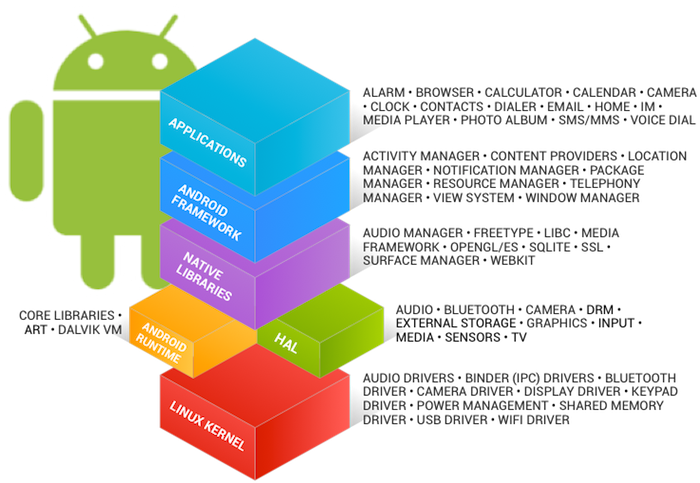
\includegraphics[width=0.8\textwidth]{android_framework_details} 
    \rule{35em}{0.5pt}
    \caption[Android-Systemarchitektur]{Die Android-Systemarchitektur Quelle: \cite{android_fig}}
    \label{fig:android}
\end{figure}
\paragraph{Linux Kernel: }
Android basiert auf dem Linux 3.14-Kernel. Dieser stellt eine bewährte Betriebssystemgrundlage dar indem er die erforderlichen Hardware-Treiber zur Verfügung stellt.
\paragraph{Android Runtime: }
Die Android Laufzeitumgebung nutzt die nachimplementierten Java-Schnittstellen \textit{aus Apache Harmony} und die Dalvik \gls{VM}. Diese wurde mit der Version 5.0 durch die Android Runtime (ART) ersetzt. \cite{android_5}
\paragraph{HAL: }
Die Andro \cite{android_hal}
\paragraph{Bibliotheken: }
Systemeigenen Bibliotheken sind C/C++ Bibliotheken und vorinstalliert. Dazu gehören alle Bibliotheken im grünen Bereich von Abbildung \ref{fig:android}:
\begin{itemize}[leftmargin=0.7cm]
\renewcommand\labelitemi{--}
	\item \textsc{Surface Manager} ~ Der für die Displayverwaltung verantwortliche Oberflächen-Manager
	\item \textsc{OpenGL/ES} ~ Eine 2D und 3D Grafikbibliothek
	\item \textsc{SGL} ~ Eine 2D Grafikbibliothek
 	\item \textsc{Media-Framework} ~ eine Medien-Bibliothek zur Wiedergabe von Audio- und Video-Daten 	
 	\item \textsc{FreeType} ~ eine Bibliothek zur Darstellung von Computerschriften als Rastergrafik
 	\item \textsc{SSL} ~ Das Secure-Socket-Layer für die Internet-Sicherheit
	\item \textsc{SQLite} ~ Ist eine ausgereifte Datenbank die den internen Gerätespeicher nutzt 
	\item \textsc{Webkit} ~ WebKit ist die Standard-Browser-Engine und erlaubt das Rendern und Anzeigen von HTML Seiten
	\item \textsc{libc} ~ Eine C-Bibliothek mit Basisfunktion
\end{itemize}
\paragraph{Application Framework: }
Androids Application-Framework ist eine Umgebung die unterschiedliche Dienste zur Verfügung stellt. Sie bietet EntwicklerInnen Zugriff auf die im Kern verwendeten \glspl{API} sowie auf die Java-Bibliotheken die für Android erstellt wurden. 
\paragraph{Applications: }
Auf der obersten Ebene in Abbildung \ref{fig:android} befinden sich die Anwendungen die den täglichen Telefon-Bedarfs wie Adressbuch, Messenger, E-Mail, Internet-Browser etc. decken. Zusätzlich unterstützt Android verschiedene Anwendungen von Drittanbietern. Diese sind hauptsächlich in Java geschrieben und werden am häufigsten über den Google Play Store verteilt.
% MOBILE SENSING
%
\subsection{Mobile Sensorik} 
Ein Sensor\footnote{ aus dem Lateinischen, deutsch: "'\textit{fühlen}"'} ist ein Bauelement, das physikalische Eigenschaften wie Helligkeit, Temperatur oder Beschleunigung sowohl quantitativ als auch qualitativ erfassen kann. Die \gls{GPS}-Sensoren in \glspl{Smartphone} sind kostengünstiger, kleiner und haben einen geringeren Stromverbrauch. Dafür allerdings eine geringere Messgenauigkeit. In der zu entwickelnden Anwendung kommt es auf jeden Meter an. Ob die Genauigkeit des integrierten \gls{GPS}-Sensors genügt, muss ergo im Rahmen dieser Arbeit getestet werden. 
% MOBILE SENSORIK UNTER ANDROID %
\subsubsection{Mobile Sensorik unter Android}
Die meisten Android-Mobilgeräte verfügen über integrierte Sensoren, die die Bewegung, Ausrichtung und verschiedene Umgebungsbedingungen messen. Diese Sensoren sind praktisch wenn man dreidimensionale Gerätbewegungen, Positionierungen oder Änderungen in der Umgebung des Gerätes überwachen möchte. So können zum Beispiel Spieleanwendungen den Beschleunigungssensor nutzen, um komplexe BenutzerInnengesten und Bewegungen wie Neigung, Erschütterung, Drehung oder Schwenkung erfassen.\\
Die Android-Plattform unterstützt Bewegungssensoren zum Messen von Beschleunigungen und Drehungen in drei Achsen, Umgebungssensoren zur Ermittlung verschiedener Umweltparameter wie Luftdruck und -feuchtigkeit, oder Beleuchtung und Temperatur, und Positionssensoren zum Messen der physikalischen Position des Gerätes. Android bietet mit dem Android Sensor Framework eine Sammlung von Klassen und Schnittstellen an mithilfe dessen man auf diese Sensoren zugreifen und deren Daten erfassen kann. \cite{android_sensor}  
%
% LOCATION BASED SERVICE
%
\subsection{Standortbezogene Dienste}
Standortbezogene Dienste (auch \gls{LBS}) sind Informationsdienste, die die geographische Position des Endgeräts nutzen, um für die NutzerInnen einen Mehrwert bereitzustellen. Sie ermöglichen den NutzerInnen den eigenen Standort zu bestimmen, zu erfahren was sich in der Nähe befindet und das (z.B. in sozialen Netzwerken) zu bewerten. Für die Bereitstellung von \gls{LBS} sind die vier Schlüsselkomponenten Mobilgerät, Content-Provider, Kommunikationsnetzwerke und Lokalisierungstechniken erforderlich. (Vgl. \cite{gps} S. 4f)\\
Zur Bestimmung von Standortdaten gibt es mehrere Techniken. Einige davon werden im Folgenden erklärt.\\ 
\textit{via NFC/Bluetooth/Sensorik?}
%
% GEOLOKATION NETWORK PROVIDER %
%
\subsubsection{Standortbestimmung via Netzwerk}
Netzwerkgestützte Standortbestimmung basiert auf Informationen des \gls{WLAN} oder der Funkzellen des Mobilfunknetzes.\\ 
% MOBILFUNK %
Funkzellentriangulierung verwendet die bekannte Geschwindigkeit von Funksignalen, um den Abstand zum Empfangsgerät zu berechnen. Das Mobilgerät muss mit einem Funkturm in Verbindung stehen. Bewegt sich das Gerät, verbindet es sich mit einem anderen Turm und die Signalstärke des sich nähernden Turms wird stärker. Unter Kenntnis der einzigartigen ID und der Position des Funkturms mit dem das Gerät verbunden ist und ggf. derer, mit denen das Gerät zuletzt verbunden war, lässt sich der eigene Standort ermitteln. (Vgl. \cite{location} S. 8f) \\
Für eine gute Lokalisierung braucht es mindestens drei, vorzugsweise vier Mobilfunkmasten oder Antennen. In Städten, wenn sich mehr Signale der Mobilfunkmasten überlappen kann eine Genauigkeit von bis zu 200 Metern erreicht werden -- bei einer geringen Funkturmdichte sinkt diese auf bis zu mehreren Kilometern, wie in Abbildung \ref{fig:cell3} illustriert. 
\begin{figure}[H]
        \centering
        \begin{subfigure}[t]{0.23\textwidth}
                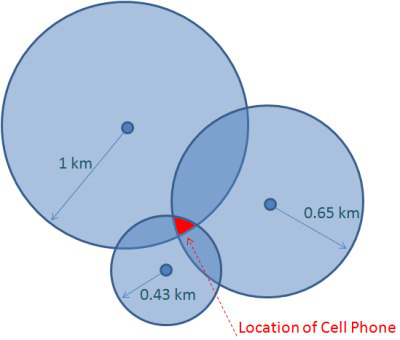
\includegraphics[width=\textwidth]{triangulation1}
                \caption{Überlappung von drei Funktürmen}
                \label{fig:cell1}
        \end{subfigure}
        ~ 
        \begin{subfigure}[t]{0.23\textwidth}
                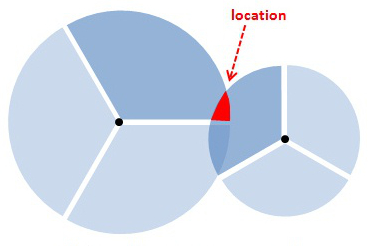
\includegraphics[width=\textwidth]{triangulation2}
                \caption{Überlappung von zwei Funktürmen mit Richtantennen}
                \label{fig:cell2}
        \end{subfigure}
         ~ 
        \begin{subfigure}[t]{0.23\textwidth}
                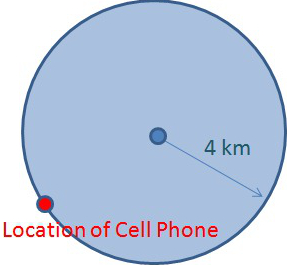
\includegraphics[width=\textwidth]{triangulation3}
                \caption{Keine Überlappung von Funkturmsignalen}
                \label{fig:cell3}
        \end{subfigure}
        \rule{35em}{0.5pt}
        \caption[Funkzellentriangulierung]{Funkzellentriangulierung Quelle: \cite{fig:cell}}
        \label{fig:cell}
\end{figure}
So eine Überlappung von drei Funktürmen ist in Abbildung \ref{fig:cell1} veranschaulicht. Diese Genauigkeit kann, wie in Abbildung \ref{fig:cell2} demonstriert, erhöht werden wenn Richtantennen auf dem Funkturm installiert sind. So kann zusätzlich die Richtung des Mobiltelefonsignals ermittelt werden. (Vgl. \cite{gps} S. 23) \\\\
%Ähnlich der funkzellenbastierten Standorterkennung funktioniert die \gls{WLAN}-basierte.
\gls{WLAN}-basierte Standorterkennung funktioniert durch Funksignale, von \gls{WLAN}-Access Points\footnote{ Drahtloser Zugangspunkt der als Schnittstelle für kabellose Kommunikationsgeräte dient} ausgesendet, um den genauen Standort eines jeden Wi-Fi-fähigen Gerätes zu ermitteln. Bei Aktivierung scannt die Software die Umgebung nach \gls{WLAN}-Access Points und berechnet die Position des Gerätes indem sie die empfangenen Signale mit der Referenzdatenbank vergleicht. Wie bei der funkzellenbastierten Standorterkennung erhöht sich auch hier die Genauigkeit (auf 20 bis 40 Meter in Europa) mit wachsender Signaldichte. \\
Effektiv werden die gleichen Prinzipien der Funkzellentriangulation übernommen. Nur werden WiFi-SSIDs\footnote{ Basic Service Set Identification (BSSID), entspricht der MAC-Adresse des Wireless Access Points oder wird als Zufallszahl erzeugt} statt Funzellenidentifikationsnummern zum Feststellen der Sendequellen verwendet. (Vgl. \cite{gps} S. 32ff) \\
Netzwerkgestützte Standortbestimmung schont zwar im Gegensatz zu \gls{GPS} den Akku und ist innerhalb von Gebäuden nutzbar, liefert jedoch wesentlich ungenauere Ergebnisse.
% GEOLIKATION GPS %
\subsubsection{Standortbestimmung via \gls{GPS}}
Die satellitengestützte Positionsbestimmung \gls{GPS} gewährleistet die Bestimmung des exakten Standpunktes und ist so wesentlicher Bestandteil ortsgebundener Anwendungen wie zum Beispiel der in Kapitel \ref{chap:state} beschriebenen. \\
\gls{GPS} wurde ursprünglich vom US-Militär entwickelt und dann Mitte der 90er Jahre der Öffentlichkeit zur Verfügung gestellt. Noch heute bleibt es mit einer Genauigkeit von bis zu vier Metern die genaueste Lokalisierungstechnologie. (Vgl. \cite{gps} S. 24f)\\
Das Globale Positionsbestimmungssystem umfasst 27 Satelliten die ständig die Erde umkreisen und dabei kontinuierlich ihre eigene, aktuelle Position und Almanach-Daten aussenden. Almanach-Daten enthalten Daten über jeden Satelliten in der Konstellation. Abbildung \ref{fig:gps} zeigt eine Darstellung der GPS-Satellitenkonstellation. Jeder Satellit folgt einer definierten Bahn, sodass mindestens vier Satelliten von jedem Standpunkt auf der Erde aus "'sichtbar"' sind. (Vgl. \cite{location} S. 4f)
\begin{figure}[H]  
    \centering  
    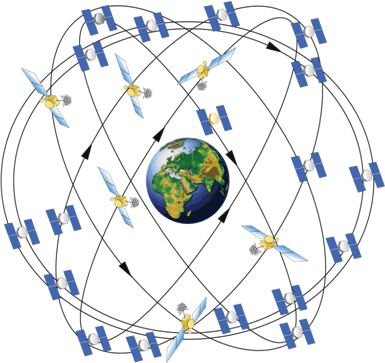
\includegraphics[width=0.4\textwidth]{gps} 
    \rule{35em}{0.5pt}
    \caption[GPS Satelliten Konstellation]{GPS Satelliten Konstellation  Quelle: \cite{fig:gps}}
    \label{fig:gps}
\end{figure}
Mittels Triangulation errechnet daraus ein \gls{GPS}-Empfänger die eigene Position. Daten von einem einzigen Satelliten lässt die Position des \gls{GPS}-Empfängers auf deinen großen Bereich der Erde einschränken. Das Hinzufügen eines zweiten engt die Position auf den Bereich, in dem sich die zwei Bereiche überlappen ein. Mit den Daten eines dritten Satelliten bekommt man bereits eine relativ genaue Positionierung. Mit jedem weiteren Satelliten wird die Präzision erhöht und durch zusätzliche Positionsinformation wie Höhe erweitert. \gls{GPS}-Empfänger benutzen regelmäßig vier bis sieben, oder gar mehr Satelliten. (Vgl. \cite{gps} S. 25f)\\
Trotzdem hat \gls{GPS}, insbesondere für mobile Plattformen einige Nachteile. Es verbraucht viel Energie, was die Akkulaufzeit des Mobiltelefons beeinträchtigt. Bevor der Standort berechnet werden kann müssen mehrere Satelliten ermittelt werden, was nach dem Kaltstart einige Zeit in Anspruch nehmen kann. (Vgl. \cite{location} S. 5)\\\\
Inzwischen wird auf etlichen Mobiltelefonen zusätzlich das russische System names Global Navigation Satellite System (GLONASS\footnote{ GLONASS, russisch Globalnaja nawigazionnaja sputnikowaja sistema, dt. Globales Satellitennavigationssystem}) eingesetzt\footnote{ \url{http://en.wikipedia.org/wiki/List_of_smartphones_supporting_GLONASS_navigation}}.
Die europäische Variante in der Testphase mit ähnlichem Aufbau heißt Galileo, die chinesische, ausschließlich inländisch genutzte, Satellitennavigation heißt BeiDou\footnote{ BeiDou, dt. Großer Bär}. (Vgl. \cite{gps} S. 24)
% A-GPS
\subsubsection{\gls{A-GPS}}
Viele moderne \glspl{Smartphone} sind heutzutage mit der \gls{GPS}-Variante \gls{A-GPS} ausgestattet. Hierbei werden Zusatzinformationen über die nächstgelegenen Satelliten via Mobilfunk bezogen, sodass sowohl die Bestimmung der Erstposition sehr viel schneller ablaufen kann. Mobilfunktürme sind oft mit einem \gls{GPS}-Empfänger ausgestattet, welche kontinuierlich die Satellitenpositionen beziehen. Diese Daten werden, sobald angefordert, an das Mobiltelefon gesendet. (Vgl. \cite{gps} S. 26f) \\
\gls{A-GPS} benötigt daher nur die Sicht auf einen Satelliten was auch genauere Ergebnisse in der Ortsbestimmung erzielt. Diese ist durch die Assistenzinformationen auch empfindlicher und somit in Städten, in denen hohe Gebäude die Sicht auf die Satelliten verdecken können, präziser.   
% GEOLOLATION UNTER ANDROID %
\subsubsection{Standortbestimmung unter Android}
Android unterstützt mit dem \texttt{android.location} Paket den Zugriff auf die Ortungsdienste. Als zentrale Komponente des Location Frameworks stellt der \texttt{LocationManager} \glspl{API} zur Lokalisierung des Geräts bereit. Mit dem \texttt{LocationManager} ist die Anwendung in der Lage alle Location Provider\footnote{ Location Provider, dt. Standortanbieter. Ein Standortanbieter bietet regelmäßige Berichte über die geographische Lage des Gerätes} des letzten bekannten Standortes abzufragen, sich für regelmäßige Updates zur Position des Gerätes anzumelden und sich wieder abzumelden wenn sich das Gerät außerhalb gegebener Parameter befindet. \cite{android_gps} \\
Die geographische Positionsangabe besteht aus Längengrad (Langitude) und Breitengrad (Lotitude). Beide werden unter anderem vom \texttt{LocationManager}-Objekt als Gleitkommawert geliefert. Daneben auch Informationen wie die Höhe in Metern über der Mehreshöhe, Peilung, Zeitstempel und die Geschwindigkeit.
\clearpage
% -------------------------------------------------
% MATHEMATISCHE GRUNDLAGEN
% -------------------------------------------------
\section{\label{sec:mathGrundlagen}Berechnung der Geschwindigkeitsempfehlung}
Präsentiert das System während der Anwendung eine Geschwindigkeitsempfehlung, ist diese abhängig von der Fahrgeschwindigkeit und vom Abstand zur Ampel. Für einen Streckenabschnitt zwischen zwei Punkten (Position der Ampel und Position der Rades) wird die Zeitspanne $\Delta t$ benötigt. Diese errechnet man mit $t_{2} - t_{1}$, woraus sich dann die Durchschnittsgeschwindigkeit im untersuchten Streckenabschnitt ergibt.\\ 
Angenommen die Progressionsgeschwindigkeit $v$ wird zum Zeitpunkt $t_{1}$ ermittelt, die \gls {LSA} schaltet zum Zeitpunt $t_{2}$ auf Rot und Abstand zur Ampel beträgt $s$, dann gilt: \\
\[ v = \frac{s}{t_{2} - t_{1}} \] \\
Der Abstand zur Ampel wird also durch die verbleibende Zeit dividiert. 
Die von der Berliner Verkehrsleitzentrale zur Verfügung gestellten Ampelsignalpläne und Position der angesteuerten Ampel sind die Basis dieser Berechnung. Die aktuelle Position des Fahrrads wird vom \gls{GPS} Sensor des \glspl{Smartphone} ermittelt und daraus der Abstand zur Ampel errechnet. Die Abbildung \ref{fig:vst} soll die Berechnungsgrundlagen veranschaulichen: 
\begin{figure}[H]  
    \centering  
    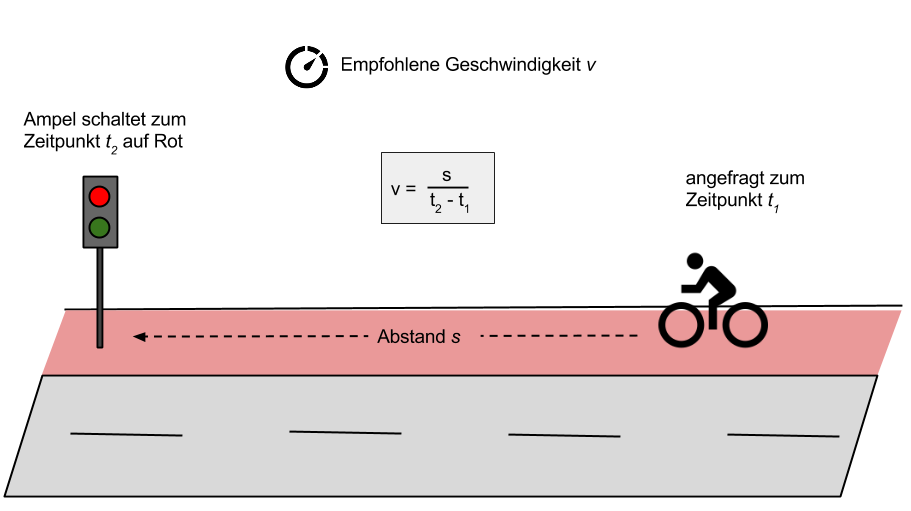
\includegraphics[width=1\textwidth]{vst}  
    \rule{35em}{0.5pt}   
    \caption[Berechnung Progressionsgeschwindigkeit]{Veranschaulichung der Berechnung}
    \label{fig:vst}
\end{figure}
Um die ensprechende \gls{LSA} während der Grünphase zu passieren, muss letztendlich die empfohlene Geschwindigkeit $v$ eingehalten werden.
